\documentclass{standalone}

\usepackage{graphicx}
\usepackage{wrapfig}
\usepackage{lscape}
\usepackage{rotating}
\usepackage{epstopdf}

\begin{document}

We have been preparing a new robot platform, Aero (Figure
\ref{fig:aero}), for use in task 2 of the challenge. From our past
experience, transportation of large robots that require to be shipped
separately proved to be very difficult due to customs regulations of
countries. 
%% It is comparatively much easier to transport a robot that
%% can be carried onto an airplane with us as carry-on luggages. 
It is comparatively much easier to transport a robot that
can be separated into modules and taken on an airplane with project personnel.
% with us as carry-on luggages. 
Aero is
designed to be light weight and modular. Compared to our HPR2 robot we
showed in our first progress report, which weighs over 80 kg, aero
only weighs approximately 65 kg. It made up of a mobile base, a
lifter, and an arm module, which can each be detached and fit into a
suitcase for transportation. 

For carrying out task 2, we have fitted Aero's arm with the same
magnetic gripper %we made for HRP2, 
described above. 

We have been considering and testing several designs of the mobile base, including the following configurations:
\begin{itemize}
	\item 4 active Mecanum wheels 
	\item 4 active tire wheels
	\item 2 	active tire wheels + 1 passive caster wheel
	\item 2 	active tire wheels + 2 passive omni wheels
\end{itemize}

Each configuration trades off maneuverability, ease of path planing,
and compatibility with different terrains. Currently we are making our
next version of the mobile base, and we will select the best
configuration for our final design based on the competition arena
ground surface type. 


\begin{figure}[h]
   \newcommand \ilenght{0.1}
   \newcommand \iheight{2.0in}
   \newcommand \iwidth{0.46\textwidth}
   \centering
   \subcaptionbox{
     \scriptsize{}\label{fig3:a}}{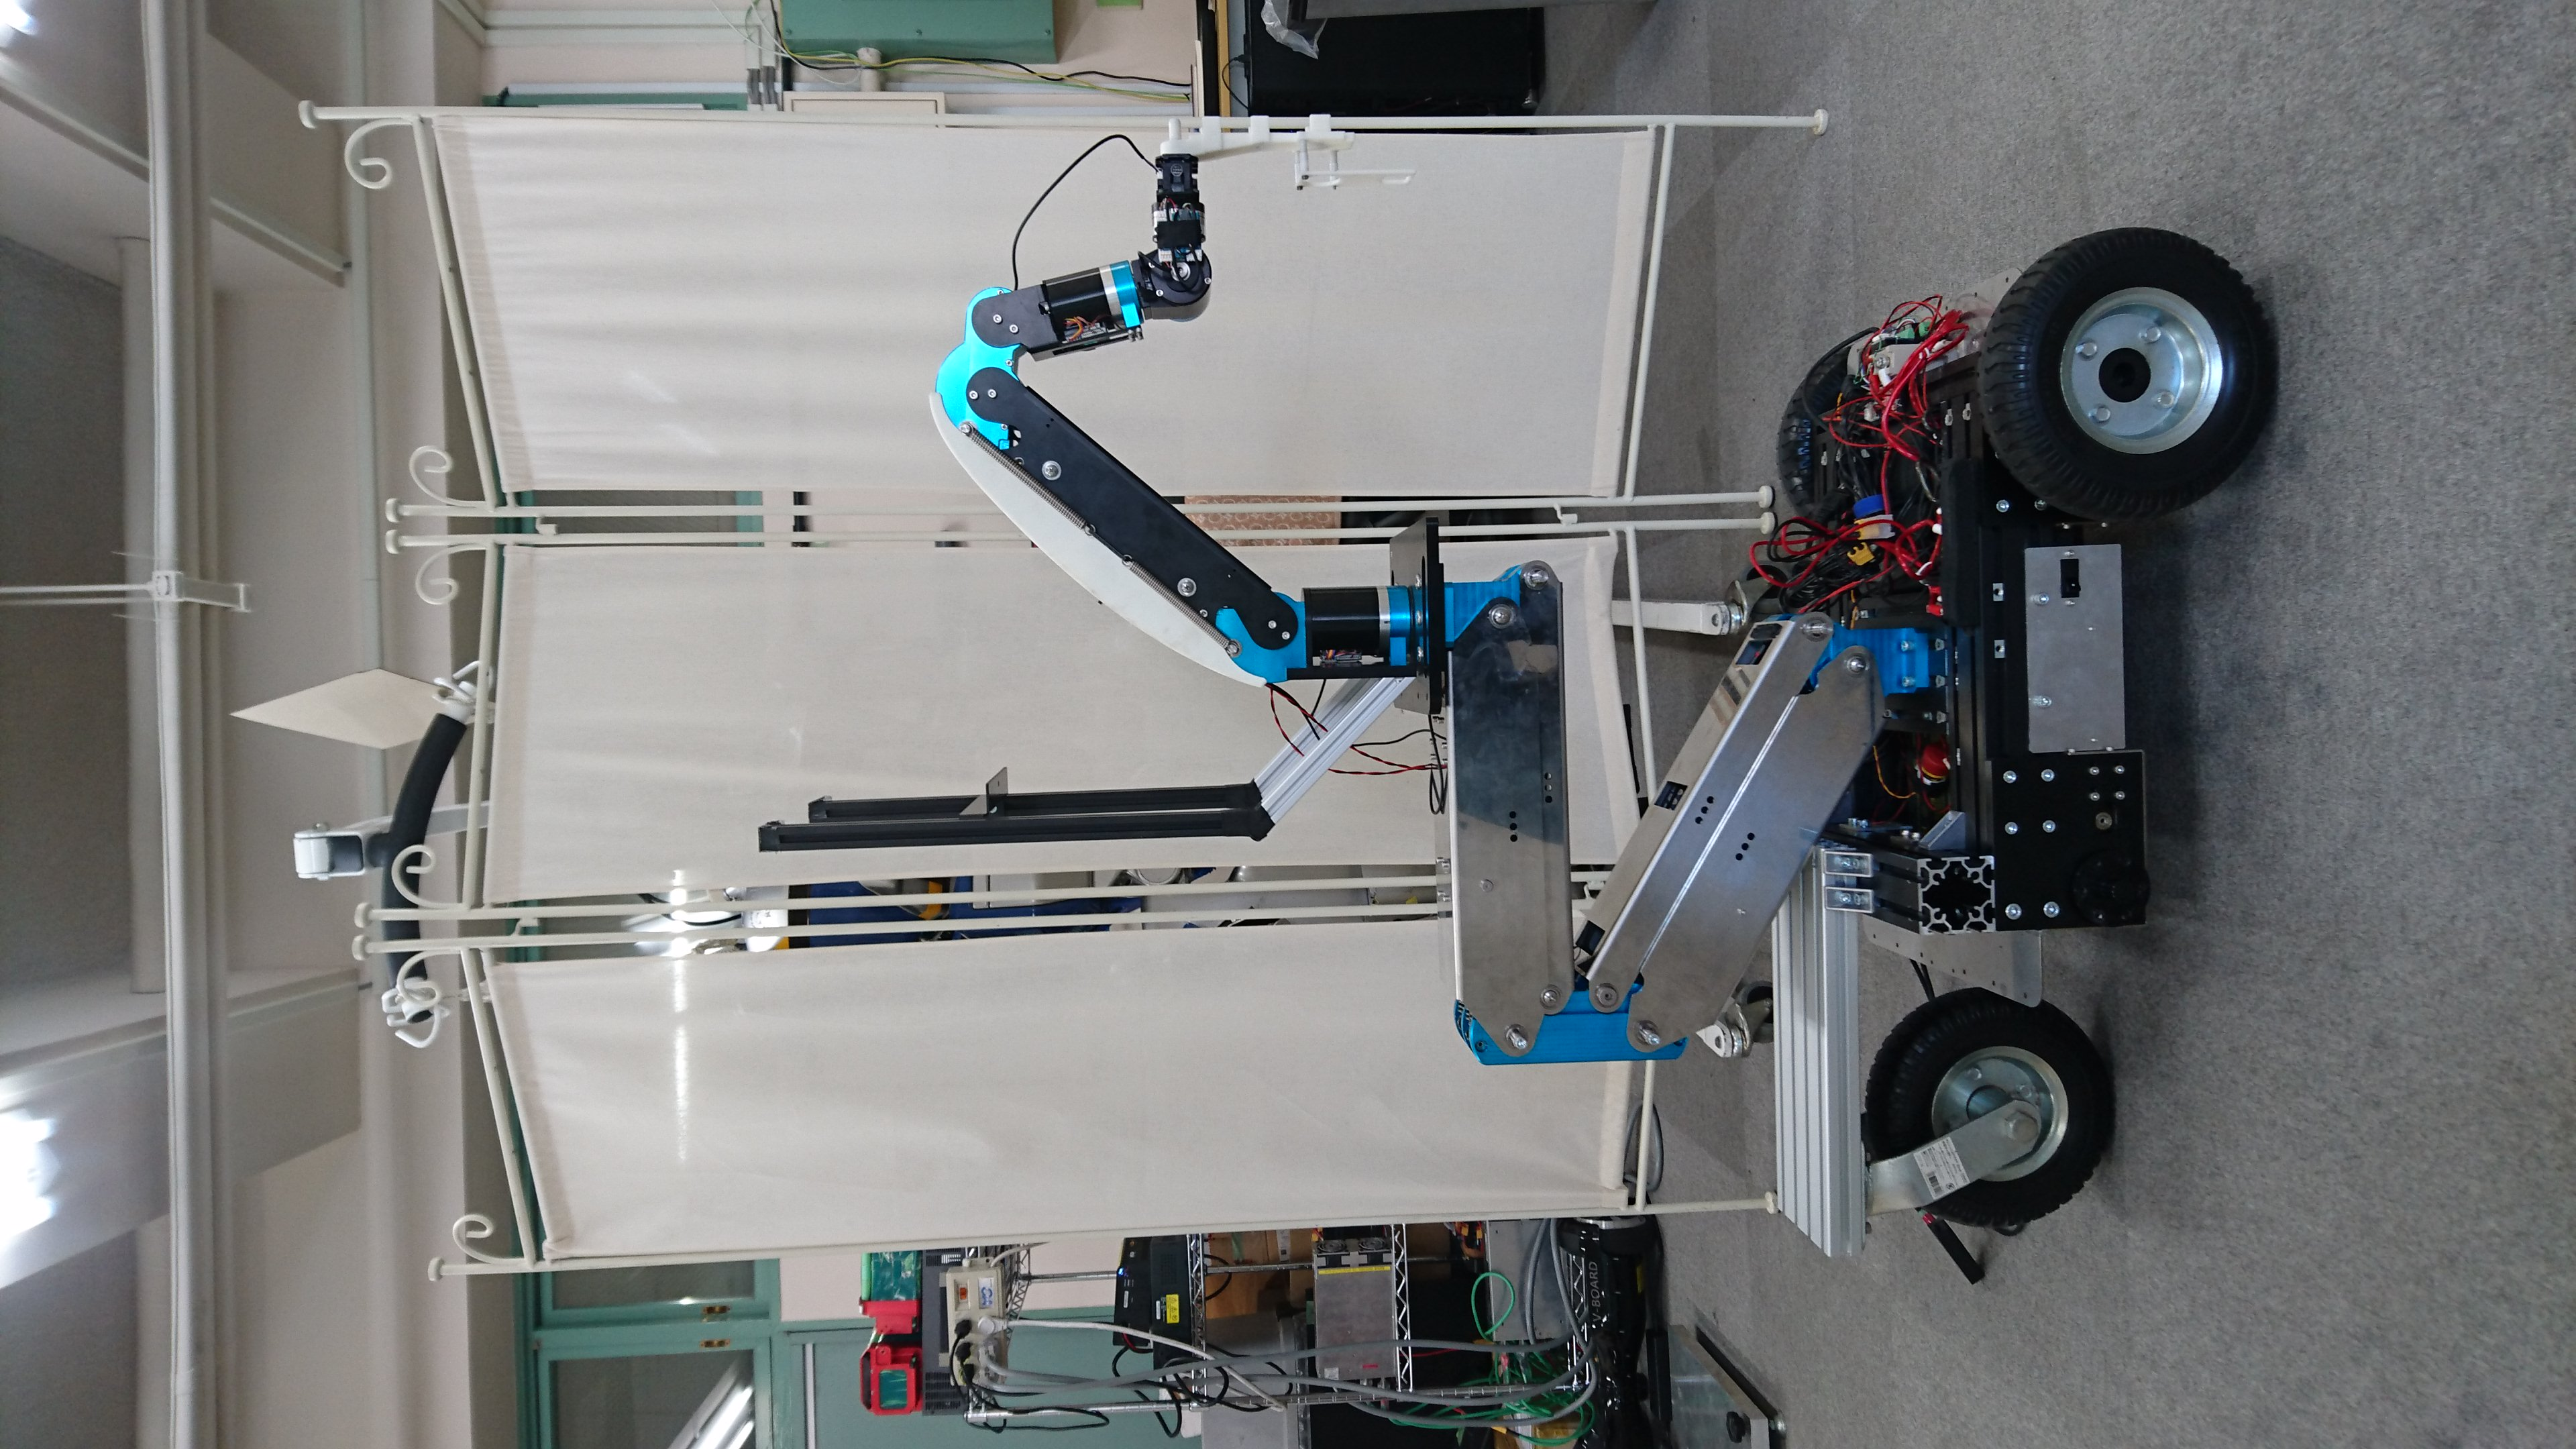
\includegraphics[width=\iwidth, height=\iheight]{sections/task2/images/aero-lowered.jpg}}\hspace{1.1em}%
   \subcaptionbox{
     \scriptsize{}\label{fig3:b}}{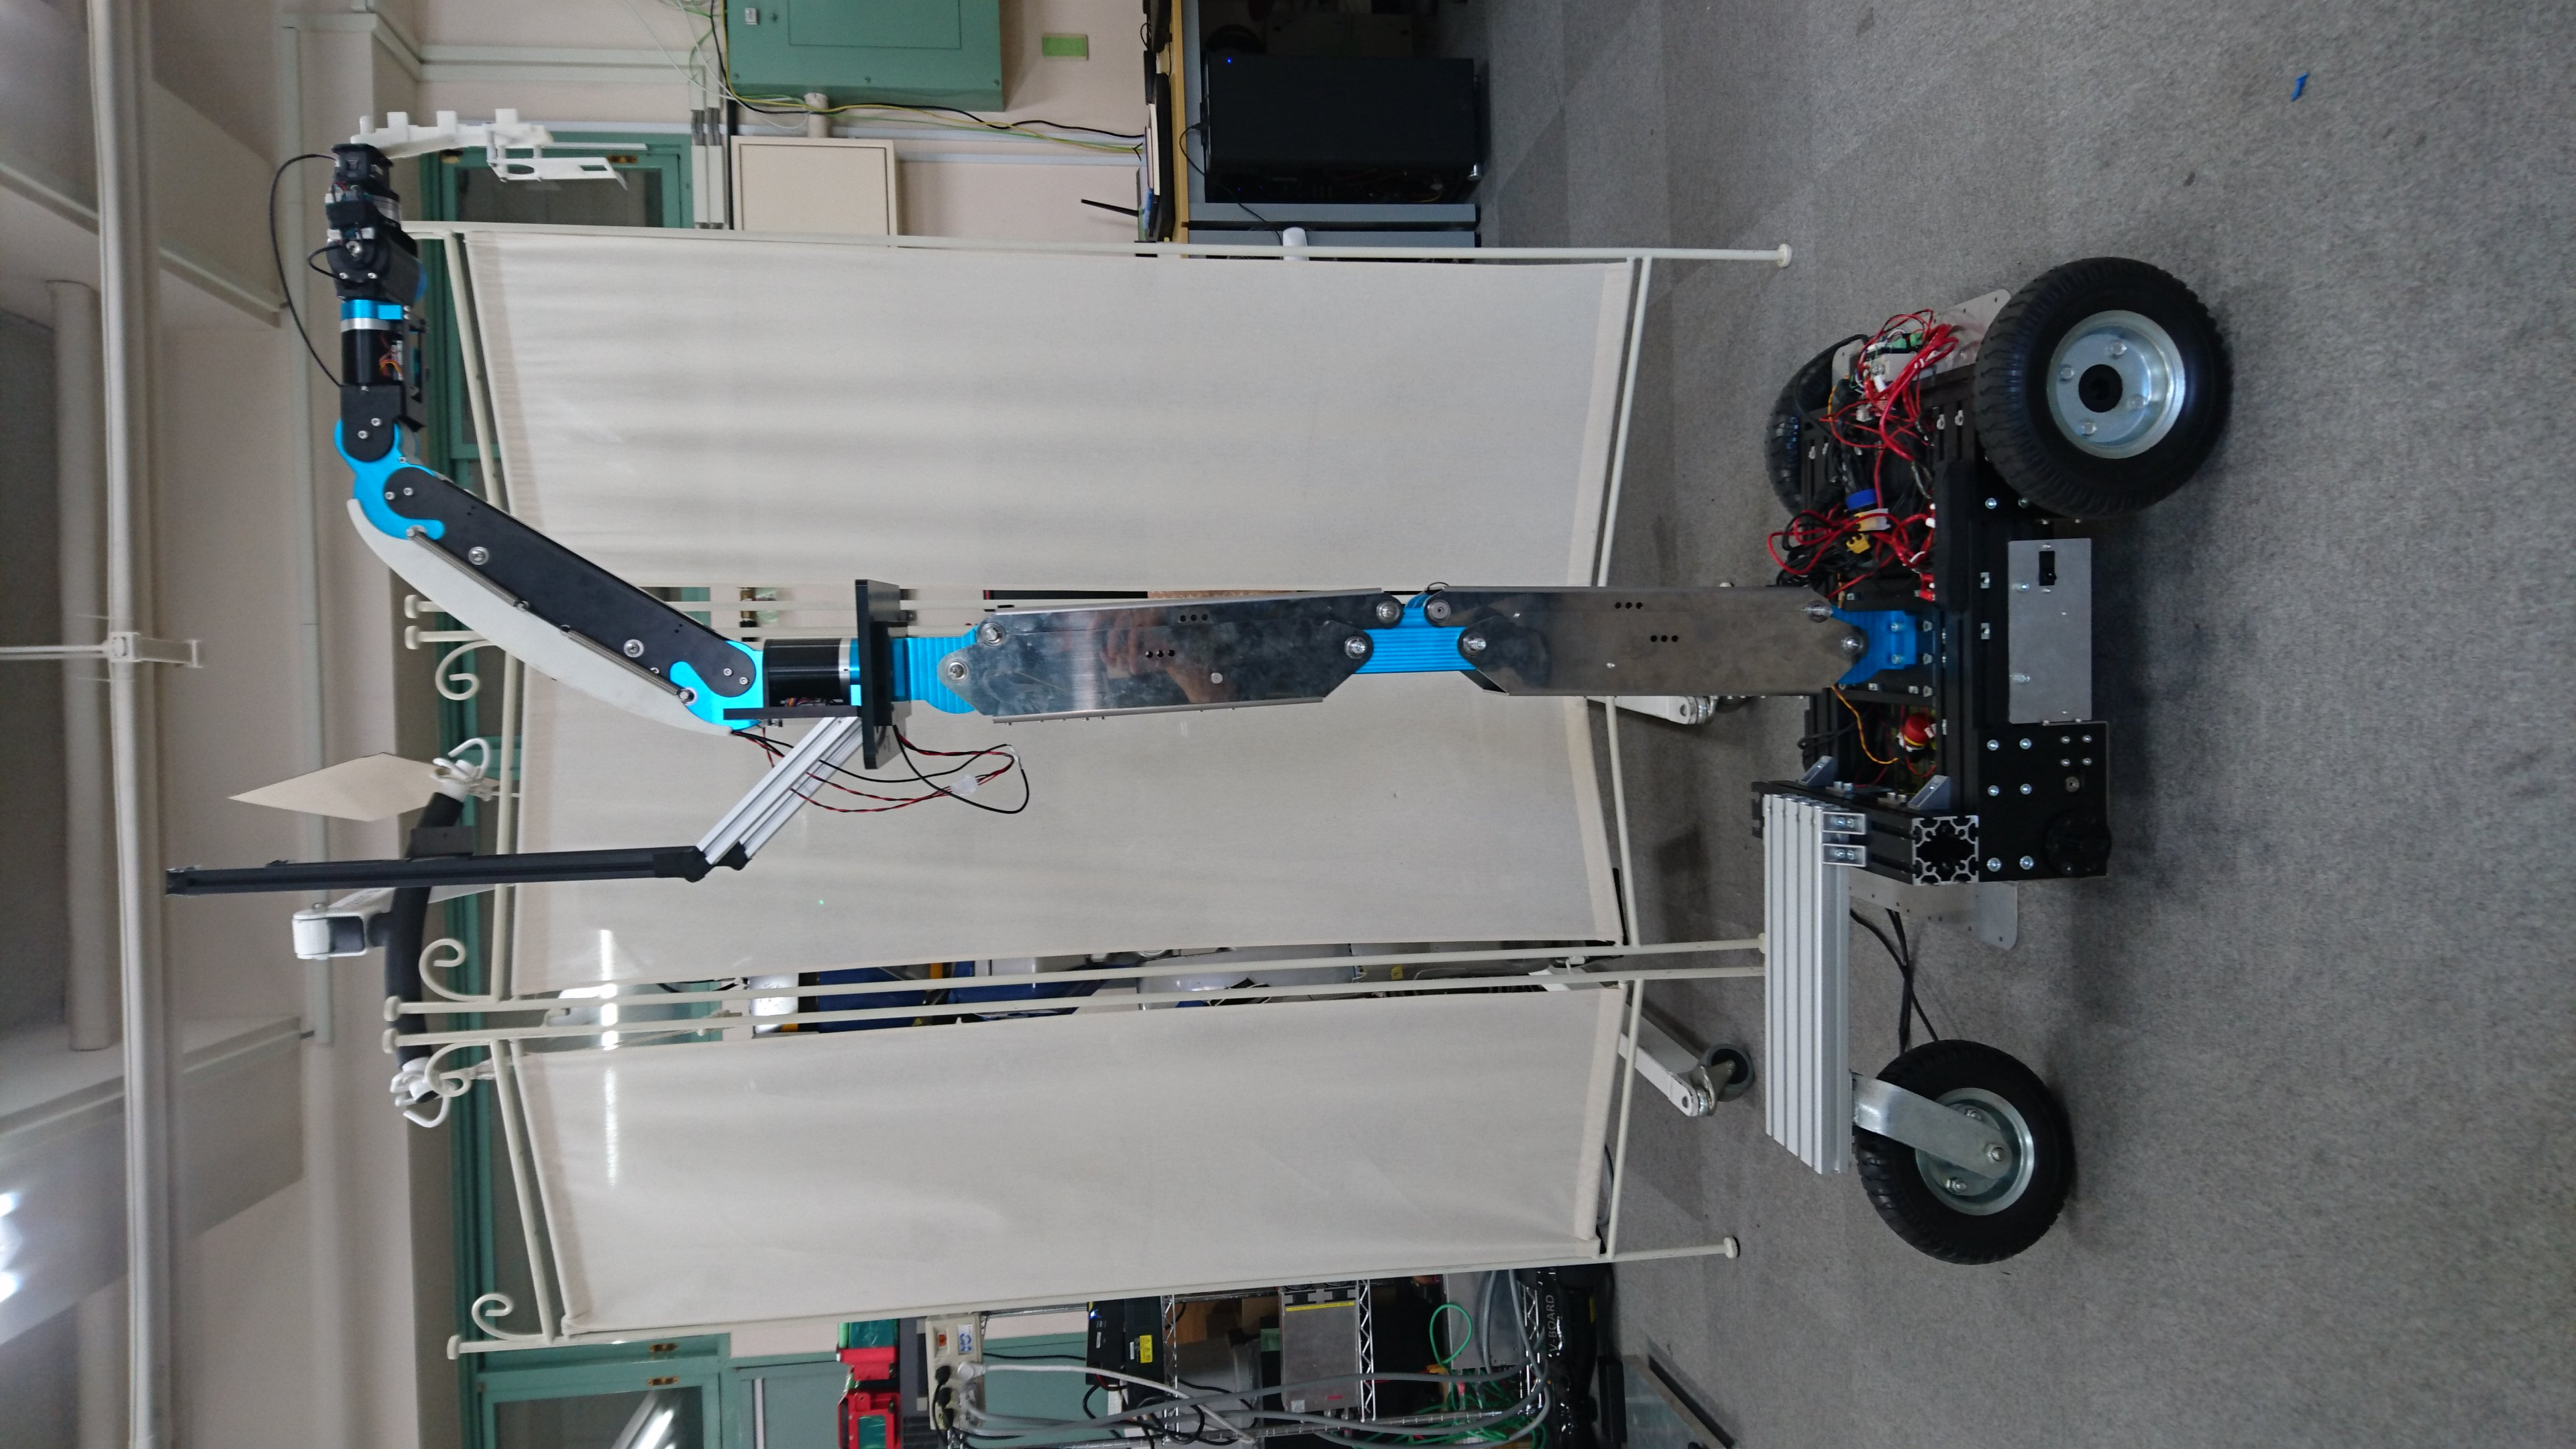
\includegraphics[width=\iwidth, height=\iheight]{sections/task2/images/aero-standup.jpg}}\hspace{1.1em}%
   \caption{Aero robot}
   \label{fig:aero}
 \end{figure}

\end{document}
